%%%%%%%%%%%%%%%%%%%%%%%%%%%%%%%%%%%%%%%%%%%%%%%%%%%%%%%%%%%%%%%
%% OXFORD THESIS TEMPLATE

% Use this template to produce a standard thesis that meets the Oxford University requirements for DPhil submission
%
% Originally by Keith A. Gillow (gillow@maths.ox.ac.uk), 1997
% Modified by Sam Evans (sam@samuelevansresearch.org), 2007
% Modified by John McManigle (john@oxfordechoes.com), 2015
%
% This version Copyright (c) 2015-2017 John McManigle
%
% Broad permissions are granted to use, modify, and distribute this software
% as specified in the MIT License included in this distribution's LICENSE file.
%

% I've (John) tried to comment this file extensively, so read through it to see how to use the various options.  Remember
% that in LaTeX, any line starting with a % is NOT executed.  Several places below, you have a choice of which line to use
% out of multiple options (eg draft vs final, for PDF vs for binding, etc.)  When you pick one, add a % to the beginning of
% the lines you don't want.


%%%%% CHOOSE PAGE LAYOUT
% The most common choices should be below.  You can also do other things, like replacing "a4paper" with "letterpaper", etc.

% This one will format for two-sided binding (ie left and right pages have mirror margins; blank pages inserted where needed):
\documentclass[a4paper,twoside]{ociamthesis}
% This one will format for one-sided binding (ie left margin > right margin; no extra blank pages):
%\documentclass[a4paper]{ociamthesis}
% This one will format for PDF output (ie equal margins, no extra blank pages):
%\documentclass[a4paper,nobind]{ociamthesis} 



%%%%% SELECT YOUR DRAFT OPTIONS
% Three options going on here; use in any combination.  But remember to turn the first two off before
% generating a PDF to send to the printer!

% This adds a "DRAFT" footer to every normal page.  (The first page of each chapter is not a "normal" page.)
\fancyfoot[C]{\emph{DRAFT Printed on \today}}  

% This highlights (in blue) corrections marked with (for words) \mccorrect{blah} or (for whole
% paragraphs) \begin{mccorrection} . . . \end{mccorrection}.  This can be useful for sending a PDF of
% your corrected thesis to your examiners for review.  Turn it off, and the blue disappears.
\correctionstrue


% Additional Packages
\usepackage{verbatim}
%\usepackage{latin}
%\usepackage{subcaption}

%%%%% BIBLIOGRAPHY SETUP

% Note that your bibliography will require some tweaking depending on your department, preferred format, etc.
% The options included below are just very basic "sciencey" and "humanitiesey" options to get started.
% If you've not used LaTeX before, I recommend reading a little about biblatex/biber and getting started with it.

% The science-type option: numerical in-text citation with references in order of appearance.
\usepackage[style=numeric-comp, sorting=none, backend=biber, doi=false, isbn=false]{biblatex}
\newcommand*{\bibtitle}{References}


% This makes the bibliography left-aligned (not 'justified') and slightly smaller font.
\renewcommand*{\bibfont}{\raggedright\small}

% Change this to the name of your .bib file (usually exported from a citation manager like Zotero or EndNote).
\addbibresource{/media/karen/dphil/Thesis/karen_thesis_2021_b/OxThesis/literature/thesis_2021.bib}





%%%%% THESIS / TITLE PAGE INFORMATION
\title{Analysis of Cellular Heterogeneity in Breast Cancer by Single Cell Sequencing}
\author{Dr. Karen Sayal}
\college{St. Cross College}

% Your full degree name.  
\degree{Doctor of Philosophy}
% Term and year of submission, or date if your board requires (eg most masters)
\degreedate{Michaelmas 2021}


%%%%% YOUR OWN PERSONAL MACROS
% This is a good place to dump your own LaTeX macros as they come up.

% To make text superscripts shortcuts
	\renewcommand{\th}{\textsuperscript{th}} % ex: I won 4\th place
	\newcommand{\nd}{\textsuperscript{nd}}
	\renewcommand{\st}{\textsuperscript{st}}
	\newcommand{\rd}{\textsuperscript{rd}}



%%%%% THE ACTUAL DOCUMENT STARTS HERE
\begin{document}



%%%%% CHOOSE YOUR LINE SPACING HERE
% This is the official option.  Use it for your submission copy and library copy:
\setlength{\textbaselineskip}{22pt plus2pt}
% This is closer spacing (about 1.5-spaced) that you might prefer for your personal copies:
%\setlength{\textbaselineskip}{18pt plus2pt minus1pt}

% You can set the spacing here for the roman-numbered pages (acknowledgements, table of contents, etc.)
\setlength{\frontmatterbaselineskip}{17pt plus1pt minus1pt}

% Leave this line alone; it gets things started for the real document.
\setlength{\baselineskip}{\textbaselineskip}


%%%%% CHOOSE YOUR SECTION NUMBERING DEPTH HERE
% You have two choices.  First, how far down are sections numbered?  (Below that, they're named but
% don't get numbers.)  Second, what level of section appears in the table of contents?  These don't have
% to match: you can have numbered sections that don't show up in the ToC, or unnumbered sections that
% do.  Throughout, 0 = chapter; 1 = section; 2 = subsection; 3 = subsubsection, 4 = paragraph...

% The level that gets a number:
\setcounter{secnumdepth}{2}
% The level that shows up in the ToC:
\setcounter{tocdepth}{2}


%%%%% ABSTRACT SEPARATE
% This is used to create the separate, one-page abstract that you are required to hand into the Exam
% Schools.  You can comment it out to generate a PDF for printing or whatnot.
\begin{abstractseparate}
	Abstract to be completed at the end.

 % Create an abstract.tex file in the 'text' folder for your abstract.
\end{abstractseparate}


% JEM: Pages are roman numbered from here, though page numbers are invisible until ToC.  This is in
% keeping with most typesetting conventions.
\begin{romanpages}

% Title page is created here
\maketitle

%%%%% DEDICATION -- If you'd like one, un-comment the following.
\begin{dedication}
This thesis is dedicated to\\
%someone\\
%for some special reason\\
\end{dedication}

%%%%% ACKNOWLEDGEMENTS -- Nothing to do here except comment out if you don't want it.
\begin{acknowledgements}
 	\subsection*{Personal}

%This is where you thank your advisor, colleagues, and family and friends.%


\subsection*{Institutional}

%If you want to separate out your thanks for funding and institutional support, I don't think there's any rule against it.  Of course, you could also just remove the subsections and do one big traditional acknowledgement section.%


\end{acknowledgements}

%%%%% ABSTRACT -- Nothing to do here except comment out if you don't want it.
\begin{abstract}
	Abstract to be completed at the end.


\end{abstract}

%%%%% MINI TABLES
% This lays the groundwork for per-chapter, mini tables of contents.  Comment the following line
% (and remove \minitoc from the chapter files) if you don't want this.  Un-comment either of the
% next two lines if you want a per-chapter list of figures or tables.
\dominitoc % include a mini table of contents
%\dominilof  % include a mini list of figures
%\dominilot  % include a mini list of tables

% This aligns the bottom of the text of each page.  It generally makes things look better.
\flushbottom

% This is where the whole-document ToC appears:
\tableofcontents

\listoffigures
	\mtcaddchapter
% \mtcaddchapter is needed when adding a non-chapter (but chapter-like) entity to avoid confusing minitoc

% Uncomment to generate a list of tables:
%\listoftables
%	\mtcaddchapter


%%% LIST OF TABLES
\listoftables

%%%%% LIST OF ABBREVIATIONS
% This example includes a list of abbreviations.  Look at text/abbreviations.tex to see how that file is
% formatted.  The template can handle any kind of list though, so this might be a good place for a
% glossary, etc.
% First parameter can be changed eg to "Glossary" or something.
% Second parameter is the max length of bold terms.
\begin{mclistof}{List of Abbreviations}{3.2cm}


\item[ER]	Oestrogen Receptor

\item[HER2]	Human Epidermal Growth Factor Receptor 2

\item[PR]	Progesterone Receptor



\end{mclistof} 


% The Roman pages, like the Roman Empire, must come to its inevitable close.
\end{romanpages}


%%%%% CHAPTERS
% Add or remove any chapters you'd like here, by file name (excluding '.tex'):
\setcounter{secnumdepth}{5}
\flushbottom
%\chapter{\label{ch:3}Single Cell RNAseq of Human Breast Cancer Cells}

\minitoc

\section{Introduction}

This document introduction won't serve as a complete primer on \LaTeX.  There are plenty of those online, and googling your questions will often get you answers, especially from \url{http://tex.stackexchange.com}.

Instead, let's talk a little about a few of the features and packages lumped into this template situation.  The \verb|savequote| environment at the beginning of chapters can add some wittiness to your thesis.  If you don't like the quotes, just remove that block.

For when it comes time to do corrections, there are two useful commands here.  First, the \verb|mccorrect| command allows you to highlight a short correction \mccorrect{like this one}.  When the thesis is typeset normally, the correction will just appear as part of the text.  However, when you declare \verb|\correctionstrue| in the main \verb|Oxford_Thesis.tex| file, that correction will be highlighted in blue.  That might be useful for submitting a post-viva, corrected copy to your examiners so they can quickly verify you've completed the task.

\begin{mccorrection}
	For larger chunks, like this paragraph or indeed entire figures, you can use the \verb|mccorrection| environment.  This environment highlights paragraph-sized and larger blocks with the same blue colour.
\end{mccorrection}

Read through the \verb|Oxford_Thesis.tex| file to see the various options for one- and two-sided printing, including or excluding the separate abstract page, and turning corrections and draft footer on or off, and the separate option to centre your text on the page (for PDF submission) or offset it (for binding).  There is also a separate option for master's degree submissions, which changes identifying information to candidate number and includes a word count.  (Unfortunately, \LaTeX has a hard time doing word counts automatically, so you'll have to enter the count manually if you require this.)

\section{Results}\label{app:imaging}


\subsection{Patient Samples and Clinical Characteristics}
I collected three patient samples at the Churchill hospital, Oxford as part of the BRECO study (REC reference 19/SC/0025) between 28th January 2020 - 23rd March 2020. BRECO is a single centre prospective study investigating the relationship between breast cancer and the surrounding tissues. Human tissue, blood samples and clinical data were collected from patients undergoing primary breast surgery. Exclusion criteria included neoadjuvant chemotherapy or radiotherapy.


My sample recruitment focused solely on ER negative, PR negative, HER2 negative invasive breast carcinoma, a rare breast cancer subtype characterised by high levels of intrinsic hypoxia. In order to facilitate sample recruitment for this rare breast cancer subtype, I was actively involved in all stages of patient identification and consent. This patient recruitment process entailed attending the home of a patient on a remote Cotswolds farm (patient consent was obtained for the home visit) or attending pre-operative surgical clinics in Horton General Hospital, Banbury.


The clinical and histological characteristics of the recruited patients are detailed in Table \ref{tab: clinical_characteristics}. Patients were identified for recruitment on the basis of ER/PR/HER2 immunohistochemistry status conducted on the diagnostic breast biopsy performed in the NHS breast cancer triple assessment clinic. All recruited patients were ER 0/8 PR 0/8 HER2 negative in the diagnostic biopsy. However, receptor status can vary when repeated on the definitive final surgical specimen.

\begin{table}[h]
	\centering
	\begin{tabular}{l | l | l}
		Study ID & TNM Stage & Hormone Receptor Status \\
		\hline
		BRECO.BC18 & pT2 50 mm pN1a (1/2) M0 & ER 2/8 PR 0/8 HER2 negative \\
		BRECO.BC20 & pT4 110 mm pN3a (33/33) M1 & ER 0/8 PR 0/8 HER2 negative \\
		BRECO.BC23 & pT3 55 mm pN1a (3/18) M0 & ER 3/8 PR 0/8 HER2 negative
	\end{tabular}
	\caption{Clinical Characteristics}
	\label{tab: clinical_characteristics}
\end{table}

\subsection{Clinical Breast Cancer Samples are amenable for Droplet-based Single Cell RNA Sequencing}
Tumour and non-tumour cells were isolated using the method detailed in chapter 2. The protocol detailed is consistent with the published literature \cite{Bassez2021}.

The key objective for the experimental single cell RNA sequencing pipeline is minimisation of the processing time to enable capture of the native cellular transcriptional state. The objective is a composite function consisting of the synergistic addition of: tissue collection, tissue dissociation to single cell suspension and single cell droplet-based encapsulation. This objective function is given high priority for clinical samples owing to the ethical and practical challenges in sample acquisition.

In the development of the single cell RNA sequencing pipeline for clinical samples, I took active measures to optimise each component. Biopsy specimens were collected intra-operatively. I collected samples directly from within the intra-operative suite and visually inspected each biopsy prior to collection. Repeat biopsies were taken by the surgical team as required.

In order to learn the techniques for single cell RNA sequencing and maximise the potential for successful sample collection, I independently established a new collaboration with Professor Xin Lu at the Ludwig Institute for Cancer Research, Oxford Branch. For all three clinical samples, I worked closely with Dr. Thomas Carroll, a DPhil student in the Lu group who has extensive experience in single cell RNA sequencing conducted as part of a completed trial in oesophageal cancer.

The cellular composition of treatment naive breast cancer, which influences therapeutic response patterns and relapse risk, is an active area of ongoing investigation. I therefore elected against marker-based selection of single cells in order to gain insight into the baseline cellular architecture.

The influence of enzymatic dissociation mixtures on final cell viability and potential bias on gene expression for clinical breast cancer samples is unclear. Therefore, during the processing of sample BRECO.BC18, I compared two enzymatic dissociation mixtures:

i. Mixture A: Collagenase D (Sigma, UK), Liberase DL (Sigma, UK) and DNase I (Sigma, UK). The unpublished protocol was shared by the group of Professor David Tuveson, Cold Spring Harbor Laboratory. This protocol has been successfully used in the dissociation of clinical pancreatic cancer samples and pancreatic cancer organoids.

ii. Mixture B: Miltenyi human tumor dissociation kit (catalogue number: 130-095-929).

Single cell encapsulation, library preparation and downstream analysis was conducted independently to compare the dissociation mixtures. The single cell clusters demonstrated little visual difference between mixture A and B (figure \ref{fig:bro18_dissociation_miltenyi_vs_cshl}). 

Therefore, I adopted dissociation mixture A, a non-propriotary cost-effective option, for all subsequently collected samples.


\begin{figure}
	\centering
	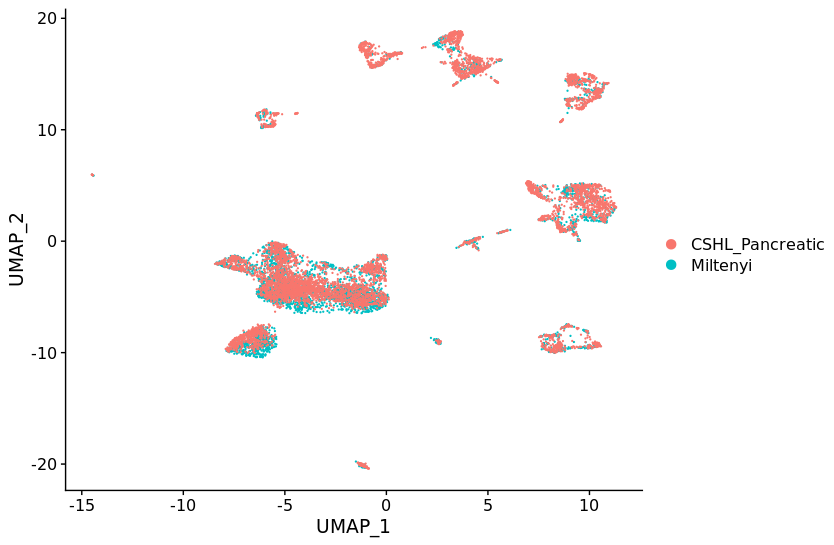
\includegraphics[width=0.7\textwidth]{figures/bro18_dissociation_miltenyi_vs_cshl.png} 
	\caption[Comparison of Dissociation Mixtures.]{UMAP depicting differences between Enzymatic Dissociation Mixtures in Sample BRECO.BC18}
	\label{fig:bro18_dissociation_miltenyi_vs_cshl}
\end{figure}



\subsection{Sample Recruitment in District General Hospitals presents Additional Challenges for the Clinical Single Cell Pipeline}

The BRECO study recruits patients within the Oxford University NHS Foundation Trust catchment area. Therefore, participant treatment can take place in the Churchill hospital, John Radcliffe hospital or Horton General hospital.

The first eligible participant, BRECO.BC15, underwent breast conserving surgery with an intra-operative research biopsy at the Horton General hospital. The geographical spread in the process, participant treatment in Banbury and laboratory facilities in Oxford, presented additional unique challenges since the experimental protocol for single cell RNA sequencing is most effective and efficient when conducted on fresh tissue. I therefore collected the biopsy directly into a vial of warmed Dmem/F12/HEPES medium supplemented with human serum which was immediately placed into a 37 \textdegree{}C water bath within a thermos flask. Mechanical dissociation was facilitated during the journey from Banbury to Oxford by gentle continual rotation of the thermos flask. The entire process required close collaboration with my colleague Miss Ashvina Segaran regarding transfer of equipment and supplies to/from Banbury and with Dr. Thomas Carroll to ensure the prompt continuation of the experimental protocol on arrival back in Oxford. Cell viability was poor at 7\% with the modified protocol and therefore, all subsequent samples were collected exclusively from the Churchill or John Radcliffe hospital.

\subsection{Cell and Gene QC is a Sample Individualised Process}
Single cell RNA seq offers the capacity to interrogate cellular heterogeneity at high resolution. A major unresolved challenge is the technical noise inherent in single cell data arising due to gene dropout, library size differences and amplification bias .



\begin{table}[h]
	\centering
	\begin{tabular}{l | l | l}
		Study ID & Median Count & Lower Threshold & Upper Threshold & Median Absolute Deviation 		\\
		\hline
		BRECO.BC18 		& 3504 & 415 & 29609 & 2.5 		\\
		BRECO.BC20.3p 	& 3243 & 384 & 27365 & 1.9 		\\
		BRECO.BC20.5p 	& 2309 & 277 & 19280 & 1.9 		\\
		BRECO.BC23 		& 1965 & 154 & 25068 & 2.95
	\end{tabular}
	\caption{Thresholds for Total Counts}
	\label{tab: qc_thesholds_counts}
\end{table}


\begin{table}[h]
	\centering
	\begin{tabular}{l | l | l}
		Study ID & Median Count & Lower Threshold & Upper Threshold & Median Absolute Deviation 		\\
		\hline
		BRECO.BC18 		& 1209 & 246 & 5934 & 2.2 	\\
		BRECO.BC20.3p 	& 1310 & 236 & 7262 & 2.25	\\
		BRECO.BC20.5p 	& 962  & 201 & 4597 & 2.2 	\\
		BRECO.BC23 		& 830  & 166 & 4158 & 2.8
	\end{tabular}
	\caption{Thresholds for Total Features}
	\label{tab: qc_thesholds_features}
\end{table}


\begin{table}[h]
	\centering
	\begin{tabular}{l | l | l}
		Study ID & Median Mitochondrial Content & Lower Threshold (\%) & Upper Threshold (\%) \\
		\hline
		BRECO.BC18 		& 7.19 & 0 & 20 \\
		BRECO.BC20.3p 	& 5.02 & 0 & 20 \\
		BRECO.BC20.5p 	& 2.58 & 0 & 16 \\
		BRECO.BC23 		& 4.77 & 0 & 20
	\end{tabular}
	\caption{Thresholds for Mitochondrial Counts}
	\label{tab: qc_thesholds_mito_percent}
\end{table}



\subsection{Unsupervised Clustering identifies Cellular Heterogeneity in Human Breast Cancer}
\label{sub:diagnostic}

Beyond the chest X-ray (`plain film'), the key non-invasive imaging modalities in diagnostic cardiology are echocardiography, magnetic resonance imaging, and X-ray computed tomography, which are reviewed below.  Nuclear medicine, including positron emission tomography (PET) and single-photon emission computed tomography (SPECT), are not discussed here, as they do not play a role in the chapters to follow.

\subsection{Characterisation of Human Breast Cancer Cellular Subtypes}







\subsection{Characterisation of Endothelial Heterogeneity in Human Breast Cancer}



\section{Discussion}

\section{Limitations}

%\include{text/ch2-litreview}
\chapter{\label{ch:3}Application of Spatial Transcriptomic Technologies in Breast Cancer}

\minitoc

\section{Introduction}


\section{Results}
%\label{app:imaging}


\subsection{Comparison of Emerging Spatial Transcriptomic Technologies}
Slide-seq
HDST
ReadCoor/FISSEQ
CARTANA
NanoString

spatial resolution vs cost vs availability



\subsection{Application of Slide-seq in Breast Cancer}
\subsubsection{Development of Slide-seq Pipeline in Breast Cancer Biopsy Samples}

After careful consideration and review of all spatial transcriptomic technologies, I elected to proceed with the use of Slide-seq on treatment naive fresh frozen breast cancer biopsies. Slide-seq is a novel technology which is not routinely available within Europe. The technology cannot be purchased from a commercial provider. At present, it is only available within the Macosko or Regev lab at the Broad Institute of MIT and Harvard, Boston, USA.


Therefore, I independently established a collaboration directly with the Macosko lab in order to proceed with this research program for my DPhil. I also established a bespoke training program within the Macosko lab for which I travelled to Boston, USA in November 2019. The training objectives were:

a. To develop expertise in the production of spatially barcoded beads and the effective uniform placement of beads onto glass slides. \\
b. To understand the process by which each bead is spatially profiled using in situ sequencing technology. \\
c. To develop best practice techniques in sample selection, tissue placement onto spatial slides and the downstream processing for library generation.

Upon completion of the training program in the US, I returned back to Oxford with a collection of pilot spatial slides to set up the novel experimental pipeline with the associated specialised reagents. The establishment of the in situ sequencing platform for the spatial slides required several years of optimisation by the Macosko lab. It would require ~ 1-2 years to develop an equivalent optimised platform in Oxford. My priority for the DPhil was to explore the application of spatial transcriptomic technologies in clinical breast cancer samples. Therefore, I aimed to establish a pipeline in which the fully profiled spatial slides would be prepared by the Macosko lab and I would process the spatial slides on clinical breast cancer samples in Oxford.

Each spatial slide, referred to as a 'puck', is produced from a 0.17 mm thick glass coverslip which is fragile. I developed expertise in the correct and gentle handling of the coverslips to avoid the creation of cracks during the protocol. Cracks created during the tissue placement stage, in particular, would introduce spatial artefacts. Consequently, the correct selection of tweezer for handling of the pucks was essential. An iterative selection process using multiple pilot slides allowed the identification of a fine stainless steel tweezer (\#T4537-1EA Sigma) as optimal for puck handling.

Slide-seq is suitable only for fresh frozen tissue. The sectioning of fresh frozen tissue is performed within a cryostat. Standard practice entails embedding tissue within OCT to provide a stable base on which sectioning is performed. However, OCT interferes with RNA hybridisation onto the puck. The placement of tissue within a cryostat must then be modified as part of the Slide-seq protocol. A small volume of OCT is placed to allow for tissue stabilisation. However, the upper layer of the tissue specimen must be kept free of OCT. 

Breast cancer clinical biopsies are \textasciitilde 4 mm diameter and of variable shape and adipose composition. The physical characteristics of the biopsies presented significant additional challenges for accurate tissue placement onto the puck. Tissue sectioning and placement was performed with Dr. Esther Bridges, a very senior and experienced scientist. The skill and technical acumen of Dr. Bridges was an essential component required for the successful establishment of the Slide-seq pipeline.


\begin{figure}[!htb]
	\minipage{0.32\textwidth}
		\left
		\includegraphics[width=0.7\textwidth, angle=270]{figures/slideseq_cryostat_1.jpg} \hfill
		\caption[Biopsy orientation in cryostat]{Biopsy \\ orientation in cryostat}
		\label{fig:slideseq_cryostat_1}
	\endminipage\hfill
	\minipage{0.32\textwidth}
		\centering
		\includegraphics[width=0.7\textwidth, angle=270]{figures/slideseq_cryostat_2.jpg} \hfill
		\caption[Sample 1]{Sample 1}
		\label{fig:slideseq_cryostat_2}
	\endminipage\hfill
	\minipage{0.32\textwidth}
		\centering
		\includegraphics[width=0.7\textwidth, angle=270]{figures/slideseq_cryostat_3.jpg} \hfill
		\caption[Sample 2]{Sample 2}
		\label{fig:slideseq_cryostat_3}
	\endminipage
\end{figure}




\subsubsection{Optimisation of Slide-seq Protocol for Application in Breast Cancer}

Xenografts
- histology images
- bioanalyzer: 45, 60, 75, 90 min


Human Samples
- histology
- bioanalyzer
- use of updated version of Slide-seq protocol.


\subsubsection{Modelling of Bead Packing Density in Slide-seq}
slides from confirmation

\subsubsection{Analysis of Slide-seq Profiling in Breast Cancer}
There is no available data to complete this section owing to the exceptional delays and disruption caused by the pandemic. 

\subsubsection{Application and Comparison of Hypoxia Signatures in Slide-seq Findings}
There is no available data to complete this section owing to the exceptional delays and disruption caused by the pandemic. 

\subsubsection{Identification of Tumour and Immune-Specific Hypoxia Markers}
There is no available data to complete this section owing to the exceptional delays and disruption caused by the pandemic. 

\subsection{Application of Single Cell Laser Capture Microdissection in Breast Cancer}
\subsubsection{Tumour and Immune Extraction in Breast Cancer at Single Cell Resolution}
There is no available data to complete this section owing to the exceptional delays and disruption caused by the pandemic. 

\subsubsection{Analysis of Single Cell RNA Sequencing}
There is no available data to complete this section owing to the exceptional delays and disruption caused by the pandemic. 

\subsubsection{Comparison of Slide-seq with Single Cell Laser Capture Microdissection in Serial Sections}
There is no available data to complete this section owing to the exceptional delays and disruption caused by the pandemic. 

\subsection{Application of In Situ Sequencing in Breast Cancer}
\subsubsection{Application of In Situ Sequencing by CARTANA on Breast Cancer}
set up MTA, OCHRe application
hypoxia signature: using published data to identify; those graphs
histology images of 

\subsubsection{Analysis of In Situ Sequencing Data in Breast Cancer}
There is no available data to complete this section owing to the exceptional delays and disruption caused by the pandemic. 

\subsection{Comparison of Expression of Hypoxia Signatures upon Spatial Transcriptomic Profiling in Breast Cancer}
There is no available data to complete this section owing to the exceptional delays and disruption caused by the pandemic. 

\section{Discussion}
I made steps to select most appropriate emerging spatial transcriptomic technology and apply these methods to clinical breast cancer samples. 
Further insights can be gained once the data is available or preliminary analysis has been completed on the available data.



\chapter{\label{ch:4}A Single Cell Atlas of Breast Cancer}

\minitoc

\section{Introduction}

This document introduction won't serve as a complete primer on \LaTeX.  There are plenty of those online, and googling your questions will often get you answers, especially from \url{http://tex.stackexchange.com}.

Instead, let's talk a little about a few of the features and packages lumped into this template situation.  The \verb|savequote| environment at the beginning of chapters can add some wittiness to your thesis.  If you don't like the quotes, just remove that block.

For when it comes time to do corrections, there are two useful commands here.  First, the \verb|mccorrect| command allows you to highlight a short correction \mccorrect{like this one}.  When the thesis is typeset normally, the correction will just appear as part of the text.  However, when you declare \verb|\correctionstrue| in the main \verb|Oxford_Thesis.tex| file, that correction will be highlighted in blue.  That might be useful for submitting a post-viva, corrected copy to your examiners so they can quickly verify you've completed the task.

\begin{mccorrection}
For larger chunks, like this paragraph or indeed entire figures, you can use the \verb|mccorrection| environment.  This environment highlights paragraph-sized and larger blocks with the same blue colour.
\end{mccorrection}

Read through the \verb|Oxford_Thesis.tex| file to see the various options for one- and two-sided printing, including or excluding the separate abstract page, and turning corrections and draft footer on or off, and the separate option to centre your text on the page (for PDF submission) or offset it (for binding).  There is also a separate option for master's degree submissions, which changes identifying information to candidate number and includes a word count.  (Unfortunately, \LaTeX has a hard time doing word counts automatically, so you'll have to enter the count manually if you require this.)

\section{Results}
%\label{app:imaging}

\subsection{Development of Single Cell Experimental Pipeline in Breast Cancer}
\subsection{Comparison of Dissociation Protocols}
\subsection{Characterisation of Major Cell Types in Breast Cancer}
\subsection{Differences in Immune Compartments in Breast Cancer}
\subsection{Characterisation of Hypoxia Markers in Immune Compartments in Breast Cancer}


\section{Discussion}

\subsection{Patient Samples and Clinical Characteristics}
I collected three patient samples at the Churchill hospital, Oxford as part of the BRECO study (REC reference 19/SC/0025) between 28th January 2020 - 23rd March 2020. BRECO is a single centre prospective study investigating the relationship between breast cancer and the surrounding tissues. Human tissue, blood samples and clinical data were collected from patients undergoing primary breast surgery. Exclusion criteria included neoadjuvant chemotherapy or radiotherapy.


My sample recruitment focused solely on ER negative, PR negative, HER2 negative invasive breast carcinoma, a rare breast cancer subtype characterised by high levels of intrinsic hypoxia. In order to facilitate sample recruitment for this rare breast cancer subtype, I was actively involved in all stages of patient identification and consent. This patient recruitment process entailed attending the home of a patient on a remote Cotswolds farm (patient consent was obtained for the home visit) or attending pre-operative surgical clinics in Horton General Hospital, Banbury.


The clinical and histological characteristics of the recruited patients are detailed in Table \ref{tab: clinical_characteristics}. Patients were identified for recruitment on the basis of ER/PR/HER2 immunohistochemistry status conducted on the diagnostic breast biopsy performed in the NHS breast cancer triple assessment clinic. All recruited patients were ER 0/8 PR 0/8 HER2 negative in the diagnostic biopsy. However, receptor status can vary when repeated on the definitive final surgical specimen.

\begin{table}
	\centering
	\begin{tabular}{l | l | l}
		Study ID & TNM Stage & Hormone Receptor Status \\
		\hline
		BRECO.BC18 & pT2 50 mm pN1a (1/2) M0 & ER 2/8 PR 0/8 HER2 negative \\
		BRECO.BC20 & pT4 110 mm pN3a (33/33) M1 & ER 0/8 PR 0/8 HER2 negative \\
		BRECO.BC23 & pT3 55 mm pN1a (3/18) M0 & ER 3/8 PR 0/8 HER2 negative \\
		\hline
	\end{tabular}
	\caption{Clinical Characteristics}
	\label{tab: clinical_characteristics}
\end{table}

\subsection{Clinical Breast Cancer Samples are amenable for Droplet-based Single Cell RNA Sequencing}
Tumour and non-tumour cells were isolated using the method detailed in chapter 2. The protocol detailed is consistent with the published literature \cite{Bassez2021}.

The key objective for the experimental single cell RNA sequencing pipeline is minimisation of the processing time to enable capture of the native cellular transcriptional state. The objective is a composite function consisting of the synergistic addition of: tissue collection, tissue dissociation to single cell suspension and single cell droplet-based encapsulation. This objective function is given high priority for clinical samples owing to the ethical and practical challenges in sample acquisition.

In the development of the single cell RNA sequencing pipeline for clinical samples, I took active measures to optimise each component. Biopsy specimens were collected intra-operatively. I collected samples directly from within the intra-operative suite and visually inspected each biopsy prior to collection. Repeat biopsies were taken by the surgical team as required.

In order to learn the techniques for single cell RNA sequencing and maximise the potential for successful sample collection, I independently established a new collaboration with Professor Xin Lu at the Ludwig Institute for Cancer Research, Oxford Branch. For all three clinical samples, I worked closely with Dr. Thomas Carroll, a DPhil student in the Lu group who has extensive experience in single cell RNA sequencing conducted as part of a completed trial in oesophageal cancer.

The cellular composition of treatment naive breast cancer, which influences therapeutic response patterns and relapse risk, is an active area of ongoing investigation. I therefore elected against marker-based selection of single cells in order to gain insight into the baseline cellular architecture.

The influence of enzymatic dissociation mixtures on final cell viability and potential bias on gene expression for clinical breast cancer samples is unclear. Therefore, during the processing of sample BRECO.BC18, I compared two enzymatic dissociation mixtures:

i. Mixture A: Collagenase D (Sigma, UK), Liberase DL (Sigma, UK) and DNase I (Sigma, UK). The unpublished protocol was shared by the group of Professor David Tuveson, Cold Spring Harbor Laboratory. This protocol has been successfully used in the dissociation of clinical pancreatic cancer samples and pancreatic cancer organoids.

ii. Mixture B: Miltenyi human tumor dissociation kit (catalogue number: 130-095-929).

Single cell encapsulation, library preparation and downstream analysis was conducted independently to compare the dissociation mixtures. The single cell clusters demonstrated little visual difference between mixture A and B (figure \ref{fig:bro18_dissociation_miltenyi_vs_cshl}). 

Therefore, I adopted dissociation mixture A, a non-propriotary cost-effective option, for all subsequently collected samples.


\begin{figure}
	\centering
	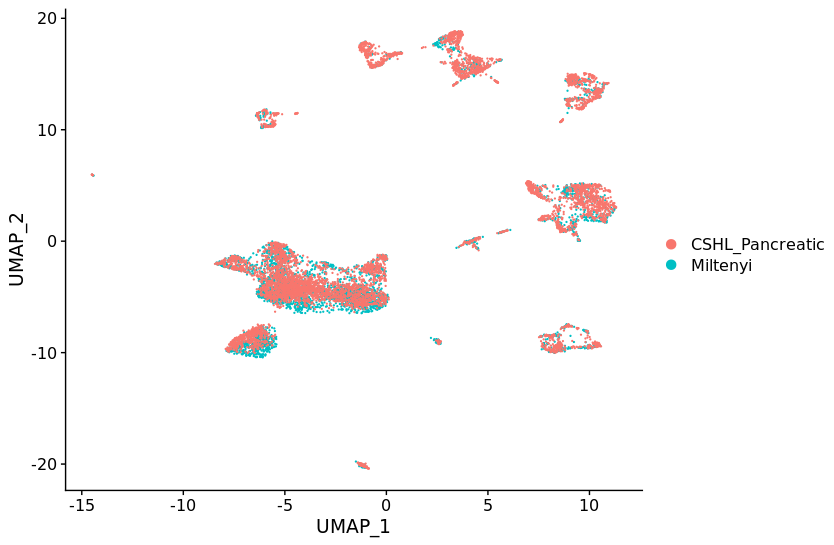
\includegraphics[width=0.7\textwidth]{figures/bro18_dissociation_miltenyi_vs_cshl.png} 
	\caption[Comparison of Dissociation Mixtures.]{UMAP depicting differences between Enzymatic Dissociation Mixtures in Sample BRECO.BC18}
	\label{fig:bro18_dissociation_miltenyi_vs_cshl}
\end{figure}



\subsection{Sample Recruitment in District General Hospitals presents Additional Challenges for the Clinical Single Cell Pipeline}

The BRECO study recruits patients within the Oxford University NHS Foundation Trust catchment area. Therefore, participant treatment can take place in the Churchill hospital, John Radcliffe hospital or Horton General hospital.

The first eligible participant, BRECO.BC15, underwent breast conserving surgery with an intra-operative research biopsy at the Horton General hospital. The geographical spread in the process, participant treatment in Banbury and laboratory facilities in Oxford, presented additional unique challenges since the experimental protocol for single cell RNA sequencing is most effective and efficient when conducted on fresh tissue. I therefore collected the biopsy directly into a vial of warmed Dmem/F12/HEPES medium supplemented with human serum which was immediately placed into a 37 \textdegree{}C water bath within a thermos flask. Mechanical dissociation was facilitated during the journey from Banbury to Oxford by gentle continual rotation of the thermos flask. The entire process required close collaboration with my colleague Miss Ashvina Segaran regarding transfer of equipment and supplies to/from Banbury and with Dr. Thomas Carroll to ensure the prompt continuation of the experimental protocol on arrival back in Oxford. Cell viability was poor at 7\% with the modified protocol and therefore, all subsequent samples were collected exclusively from the Churchill or John Radcliffe hospital.

\subsection{Cell and Gene QC is a Sample Individualised Process}
Single cell RNA sequencing offers the capacity to interrogate cellular heterogeneity at high resolution. A major unresolved challenge is the technical noise inherent in single cell data arising due to dropout events, library size differences and amplification bias \cite{Eraslan2019}. A dropout event occurs when an expressed gene fails to be detected due to low RNA capture rates. Dropout events are distinct to a 'true biological' zero count which, in contrast, is a faithful representation of the native transcriptional state \cite{Eraslan2019}. The distinction between a 'true' and 'false' zero count has yet to be clearly defined. Therefore, traditional imputation methods used to correct for missing values may not be suitable for scRNA-seq data.

A range of alternative approaches for quality control (QC) are being explored. These methods include using:
i. Spike-in molecules
ii. Housekeeping genes 
iii. Library size correction

i. Spike-in Normalisation
Spike-in molecules consist of RNA artificially added to each cell lysate in the same volume. Therefore, variations in concentration will be similar between endogenous and spike-in molecules between samples \cite{Katayama2013}. The spike-in concentration is known a priori which then allows for the generation of spike-in normalisation factors to correct for global changes between samples \cite{Katayama2013}. Spike-in normalisation is suitable for plate-based single cell technologies such as Smart-seq2. There is no comparable method available for droplet-based single cell techniques, such as the 10X Chromium system used for my single cell breast cancer samples. Spike-in normalisation was therefore not a viable option for my experimental design.

ii. Housekeeping Genes
Housekeeping (HK) genes, such as \textbf{GAPDH} and \textbf{ACTB}, are genes which are required for basic cellular function. HK genes have been explored as potential single cell QC markers under the assumption that they are highly and consistently expressed between good quality samples. This assumption holds true in bulk RNA-seq studies with HK genes demonstrating an uniform expression distribution. However, single cell qPCR has demonstrated high variation in HK gene expression between single endodermal cells derived from human embryonic stem cells \cite{Oyolu2012}. Therefore, selection of single cells based on HK gene expression may result in loss of true biological variation.

iii. 

\begin{table}[ht]
	\centering
	\small
	\renewcommand{\arraystretch}{1.4}
	{\columnwidth}{5}
	\begin{tabular}{|l| c | c | c | c |}
		\hline
		Study ID	&	Median Count & Lower Threshold & Upper Threshold & Median Absolute Deviation \\
		\hline
		BRECO.BC18 		& 3504 & 415 & 29609 & 2.5 	\\
		
		BRECO.BC20.3p 	& 3243 & 384 & 27365 & 1.9 		\\
		
		BRECO.BC20.5p 	& 2309 & 277 & 19280 & 1.9 		\\
		
		BRECO.BC23 		& 1965 & 154 & 25068 & 2.95\\
		\hline
	\end{tabular}
	\caption{Thresholds for Total Counts}
	\label{tab: qc_thesholds_counts}
\end{table}


\begin{table}[ht]
	\centering
	\small
	\renewcommand{\arraystretch}{1.4}
	\begin{tabular}{| l | c | c | c | c |}
		\hline
		Study ID	&	Median Features & Lower Threshold & Upper Threshold & Median Absolute Deviation \\
		\hline
		BRECO.BC18 		& 1209 & 246 & 5934 & 2.2 	\\
		BRECO.BC20.3p 	& 1310 & 236 & 7262 & 2.25	\\
		BRECO.BC20.5p 	& 962  & 201 & 4597 & 2.2 	\\
		BRECO.BC23 		& 830  & 166 & 4158 & 2.8	\\
		\hline
	\end{tabular}
	\caption{Thresholds for Total Features}
	\label{tab: qc_thesholds_features}
\end{table}

\begin{table}
	\centering
	\small
	\renewcommand{\arraystretch}{1.4}
	\begin{tabular}{| l | c | c | c | c |}
		\hline
		Study ID & Median Mitochondrial Content & Lower Threshold (\%) & Upper Threshold (\%) \\
		\hline
		BRECO.BC18 		& 7.19 & 0 & 20 \\
		BRECO.BC20.3p 	& 5.02 & 0 & 20 \\
		BRECO.BC20.5p 	& 2.58 & 0 & 16 \\
		BRECO.BC23 		& 4.77 & 0 & 20 \\
		\hline
	\end{tabular}
	\caption{Thresholds for Mitochondrial Counts}
	\label{tab: qc_thesholds_mito_percent}
\end{table}




\subsection{Unsupervised Clustering identifies Cellular Heterogeneity in Human Breast Cancer}
\label{sub:diagnostic}

Beyond the chest X-ray (`plain film'), the key non-invasive imaging modalities in diagnostic cardiology are echocardiography, magnetic resonance imaging, and X-ray computed tomography, which are reviewed below.  Nuclear medicine, including positron emission tomography (PET) and single-photon emission computed tomography (SPECT), are not discussed here, as they do not play a role in the chapters to follow.

\subsection{Characterisation of Human Breast Cancer Cellular Subtypes}







\subsection{Characterisation of Endothelial Heterogeneity in Human Breast Cancer}



\section{Discussion}

\section{Limitations}

\chapter{\label{ch:5}Integration of Single Cell Atlas with Slide-seq Profiling in Breast Cancer}

\section{Introduction}
The intention for my final results chapter was to integrate dissociated single cell sequencing data with spatial transcriptomic data in breast cancer in order to provide insight on spatially distinct transcriptional profiles which could guide future therapeutic development.


\section{Results}

\subsection{Integration of Paired Single Cell Profiling with Slide-seq Profiling in Breast Cancer}
The production of Slide-seq data has been delayed during the pandemic. I have made exhaustive efforts to make progress on this work within the time-frame of my DPhil. The data has not been available in time for exploration as part of my thesis. There is no published Slide-seq cancer data to provide guidance on potential insight or intended results. It has therefore not been possible to complete this section owing to the exceptional delays and disruption caused by the pandemic. 

\subsection{Identification of spatially Distinct Transcriptional Responses Conserved amongst Different Patient Samples}
Data required for the completion of this section is pending owing to the exceptional delays and disruption caused by the pandemic. 

\subsection{Integration of Slide-seq Profiling with an Unpaired Single Cell Atlas}
Data required for the completion of this section is pending owing to the exceptional delays and disruption caused by the pandemic. 

\subsection{Comparison of Different Single Cell Atlases in Breast Cancer and Integration with Slide-seq Profiling}
Data required for the completion of this section is pending owing to the exceptional delays and disruption caused by the pandemic. 

\section{Discussion}
Once available, the results will warrant analysis to provide insight on spatially profiled gene expression in clinical breast cancer.







%% APPENDICES %% 
% Starts lettered appendices, adds a heading in table of contents, and adds a
%    page that just says "Appendices" to signal the end of your main text.
%\startappendices
% Add or remove any appendices you'd like here:
%\include{text/appendix-1}


%%%%% REFERENCES

% JEM: Quote for the top of references (just like a chapter quote if you're using them).  Comment to skip.

\setlength{\baselineskip}{0pt} % JEM: Single-space References

{\renewcommand*\MakeUppercase[1]{#1}%
\printbibliography[heading=bibintoc,title={\bibtitle}]}


\end{document}
